\documentclass[]{beamer}
\usepackage{xmpmulti}
\usepackage{psfrag}
\usepackage{xcolor}
\usepackage{chessboard}
\newcommand{\owner}{\mathcal{O}}
\newcommand{\manager}{\mathcal{M}}

\usepackage{tikz}
\usetikzlibrary{snakes}
\usetikzlibrary{backgrounds} 
\usepackage{pgfmath}


\mode<presentation>
{\usetheme{Boadilla}  % very plain
}

\usepackage{xcolor}

\usepackage{amssymb,amsmath,amsthm}
\usepackage{boxedminipage}

\setbeamercolor{uppercol}{fg=teal,bg=lightgray}%
\setbeamercolor{lowercol}{fg=olive,bg=lightgray!50}%

\newcommand{\curr}{\mathtt{current}}
\newcommand{\mos}{\mathtt{m}}
\newcommand{\move}{\mathtt{lmove}}
\newcommand{\nmove}{\mathtt{nmove}}

\title[]{Certificates with OpenSSL}

\author{Giuseppe Persiano}

\institute[UNISA]{%
Universit\`a di Salerno\\ \qquad \\
}

\date[November 2020]{November, 2020}

\begin{document}

\begin{frame}
  \titlepage
\end{frame}
\begin{frame}
\frametitle{Two-Level CA}
\begin{block}{Two-Level CA}
\begin{itemize}
\item  One {\em Root CA} that produces certificats for the 
{\em Intermediate CA}

\vskip .3cm

\item One or more {\em Intermediate CA}s that produce certificates for {\em clients} and {\em servers}
\end{itemize}
\end{block}
\end{frame}

\begin{frame}
\frametitle{Setting up the folder for a CA}

The CA needs the following directories:
\begin{itemize}
    \item {\tt certs}: to store own certificate
    \item {\tt private}: to store own private key
    \item {\tt newcerts}: to store signed certificates indexed
        by serial number
    \item {\tt crl}: to store the certificate revocation lists
    \item {\tt csr}: to store the certificate signing requests
\end{itemize}
\vskip .4cm
and the following files
\begin{itemize}
    \item {\tt serial}: holds the serial number of the next
        certificate
    \item {\tt index.txt}: DNs of the signed certificates
\end{itemize}
\end{frame}

\begin{frame}
\frametitle{Setting up the Root Certificate}

\begin{block}{Root CA}
A two-step process:
\begin{itemize}
\item Generate the private key

    {\color{brown} \tt openssl genrsa -aes256 -out private/cakey.pem 4096}

    {\color{red} Protect the private key by making it readable only to owner}

\item Produce the certificate by signing the public key

    Self-sign the public key with the command

    {\color{brown} \tt openssl req -new}
    \begin{itemize}
        \item {\tt -x509} self signed
        \item {\tt -config} the configuration file to be used
        \item {\tt -extensions} the section of the configuration file 
    \end{itemize}
    {\color{red} Protect the certificate by making it only readable }


\end{itemize}
\end{block}

See script {\tt createRootCert.sh}
\end{frame}

\begin{frame}
\frametitle{What is in the Root CA}
\begin{center}
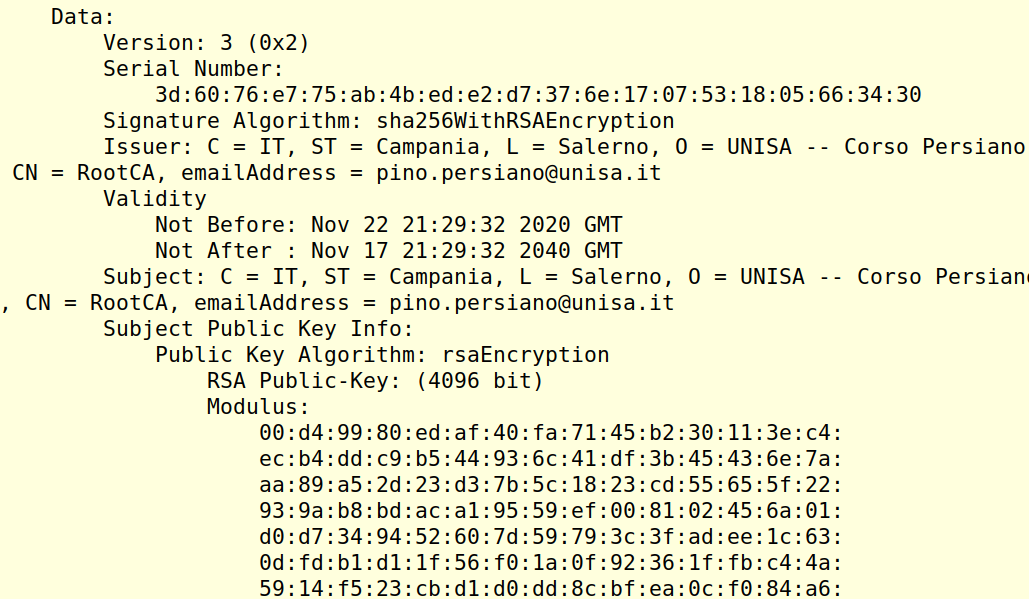
\includegraphics[width=3.5in]{imgs/rootCert.png}
\end{center}
\end{frame}

\begin{frame}
\frametitle{Setting up the Intermediate Certificate}
\begin{block}{Intermediate CA: a three-step process}
\begin{itemize}
\item Generate the private key {\tt [createIntermediate.sh]}

    {\color{brown} \tt openssl genrsa -aes256 -out private/cakey.pem 4096}

    {\color{red} Protect the private key by making it readable only to owner}

\item Generate a Certificate Signing Request for the Root CA
{\tt [createIntermediate.sh]}

    {\color{brown} \tt openssl req}

    \begin{itemize}
        \item {\tt -config} specifies the configuration file to be used
        \item {\tt -key} specifies the key to be certified
        \item {\tt -out} file containing the CSR output
    \end{itemize}

\item Sign the CSR using the Root CA private key 
{\tt [signIntermediate.sh]}

    {\color{brown} \tt openssl ca}
    \begin{itemize}
        \item {\tt -config} configuration file 
        \item {\tt -extensions} section of the configuration file
    \end{itemize}

    Create the chain of certificates:

        concatenate the new certificate and the root's 
            self-signed certificate


\end{itemize}

\end{block}
\end{frame}

\begin{frame}
\frametitle{Verifying the intermediate certificate}

\centerline{\color{magenta} \tt openssl verify -CAfile RootCert IntermediateCert}

\begin{center}
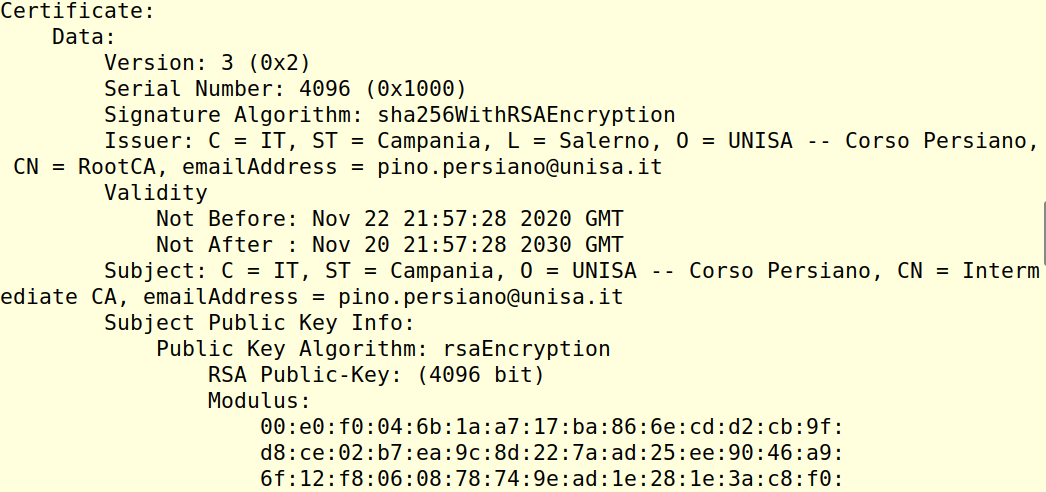
\includegraphics[width=3.5in]{imgs/intermediateCert.png}
\end{center}
\end{frame}

\begin{frame}
\frametitle{Producing certificates}
\begin{block}{Client certificate: a three-step process}
\begin{itemize}
\item Generate the private key {\tt [createClient.sh]}

    {\color{brown} \tt openssl genrsa -aes256 -out aa@aa.com.key.pem 2048}

\item Generate a Certificate Signing Request for the Intermediate CA
{\tt [createClient.sh]}

    {\color{brown} \tt openssl req}

    \begin{itemize}
        \item {\tt -config} specifies the configuration file to be used
        \item {\tt -key} specifies the key to be certified
        \item {\tt -out} file containing the CSR output
    \end{itemize}

\item Sign the CSR using the Intermediate CA private key 
{\tt [createClient.sh]}

    {\color{brown} \tt openssl ca}
    \begin{itemize}
        \item {\tt -config} configuration file 
        \item {\tt -extensions} section of the configuration file
            
            use the  user section or the server section 
    \end{itemize}

\end{itemize}
\end{block}
\end{frame}

\begin{frame}
\frametitle{Inspecting the client certificate}

\centerline{\color{magenta} \tt openssl x509 -noout -text -in certs/aa@aa.com.cert.pem}

\begin{center}
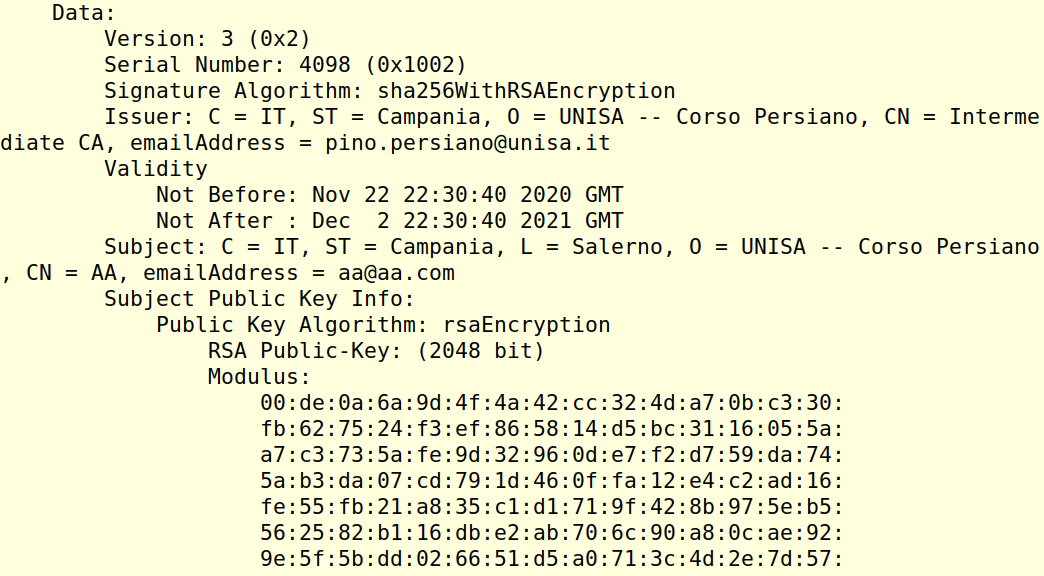
\includegraphics[width=3.5in]{imgs/clientCert.png}
\end{center}
\end{frame}

\begin{frame}
\frametitle{Inspecting the client certificate}

\centerline{\color{magenta} \tt openssl x509 -noout -text -in certs/aa@aa.com.cert.pem}

\begin{center}
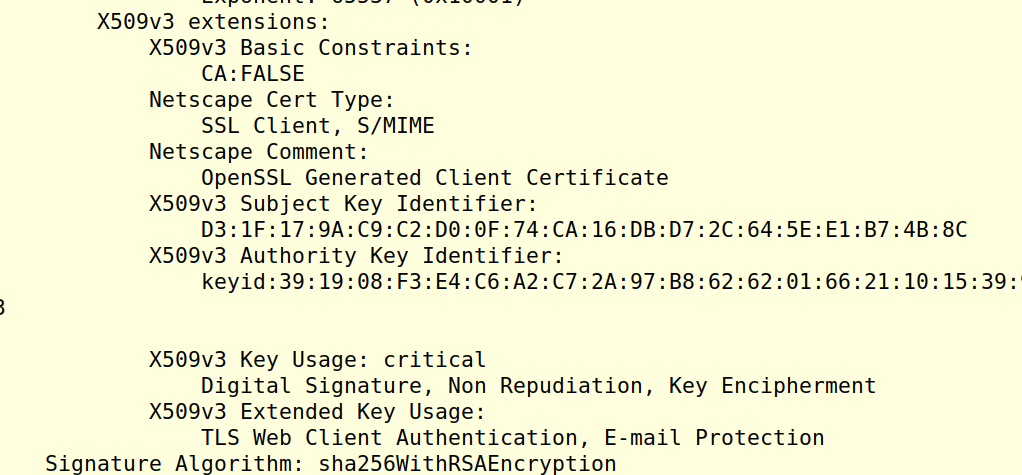
\includegraphics[width=3.5in]{imgs/clientCert2.png}
\end{center}
\end{frame}

\begin{frame}
\frametitle{Inspecting the server certificate}

\centerline{\color{magenta} \tt openssl x509 -noout -text -in certs/www.example.com.cert.pem}

\begin{center}
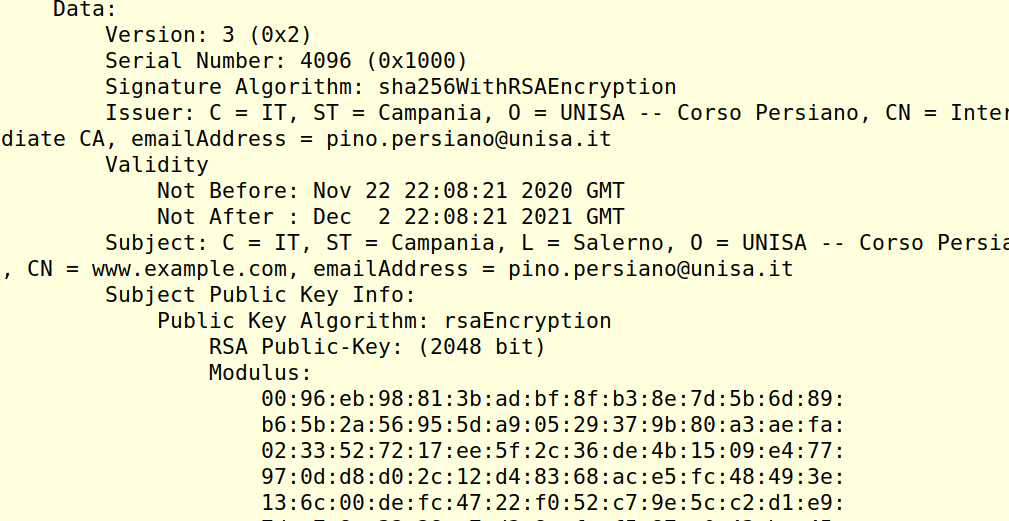
\includegraphics[width=3.5in]{imgs/serverCert.png}
\end{center}
\end{frame}

\begin{frame}
\frametitle{Inspecting the server certificate}

\centerline{\color{magenta} \tt openssl x509 -noout -text -in certs/www.example.com.cert.pem}


\begin{center}
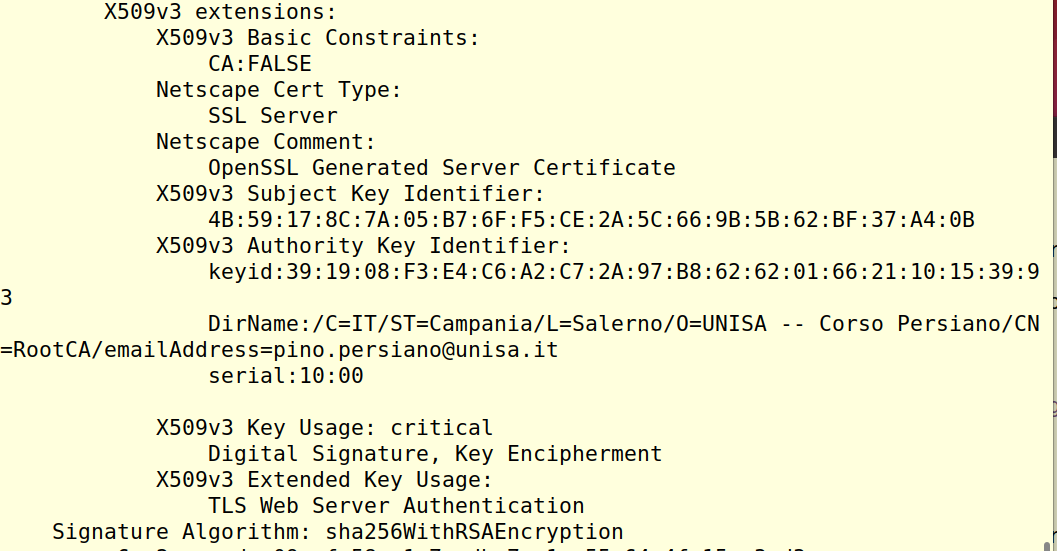
\includegraphics[width=3.5in]{imgs/serverCert2.png}
\end{center}
\end{frame}


\end{document}
